%------------------------------------------------------------
\subsection{Introduction}


%------------------------------------------------------------
\begin{frame}{Introduction}

\begin{center}
A (not-so-uncommon) nightmare

\includegraphics[width=12cm]{02_encapsulation/figures/nightmare.pdf}

What changed?
\end{center} \pause

\begin{itemize}
  \item Software version
  \item Libraries version
  \item OS version
  \item ..?
\end{itemize}

\end{frame}


%------------------------------------------------------------
\subsection{Different levels of encapsulation}

%------------------------------------------------------------
\begin{frame}{Different levels of encapsulation}


Goal : capture the system environment of applications (OS, packages, libraries,…) to control their execution.

\begin{itemize}
  \item Hardware virtualisation (virtual machines) \logoVirtualbox 
  \item OS virtualisation (images and containers) \logoDockerPortrait
  \item Environment management \logoConda
\end{itemize}

\end{frame}

%------------------------------------------------------------
\begin{frame}{Encapsulation}

Let's say we want to install Firefox...

\includegraphics[width=12cm]{02_encapsulation/figures/install_firefox.pdf}


\end{frame}

%------------------------------------------------------------
\begin{frame}{Encapsulation}
\begin{columns}

\column{0.5\textwidth}
\includegraphics[width=6cm]{02_encapsulation/figures/install_firefox.pdf}

\column{0.5\textwidth}
We started with a computer using a specific OS...


And inside this environment, we installed a new application.


Applications rely on dependencies, e.g. external libraries.

\end{columns}
\end{frame}

%------------------------------------------------------------
\begin{frame}{Encapsulation}
\begin{columns}

\column{0.5\textwidth}
\includegraphics[width=6cm]{02_encapsulation/figures/install_firefox.pdf}

\column{0.5\textwidth}
Usually dependencies of different applications don’t interfere.


But what if we want to test the latest version of our favourite tool?
There might be conflicts…

\end{columns}
\end{frame}

%------------------------------------------------------------
\begin{frame}{Encapsulation : hardware virtualisation}
\begin{columns}

\column{0.5\textwidth}
\includegraphics[width=6cm]{02_encapsulation/figures/install_firefox.pdf}

\column{0.5\textwidth}
Idea: use virtual machines

Pros: 
\begin{itemize}
  \item Each application gets a completely different and independent environment
  \item Virtual machines can be transferred to another computer (using the same manager)
\end{itemize}

\end{columns}
\end{frame}

%------------------------------------------------------------
\begin{frame}{Encapsulation : hardware virtualisation}

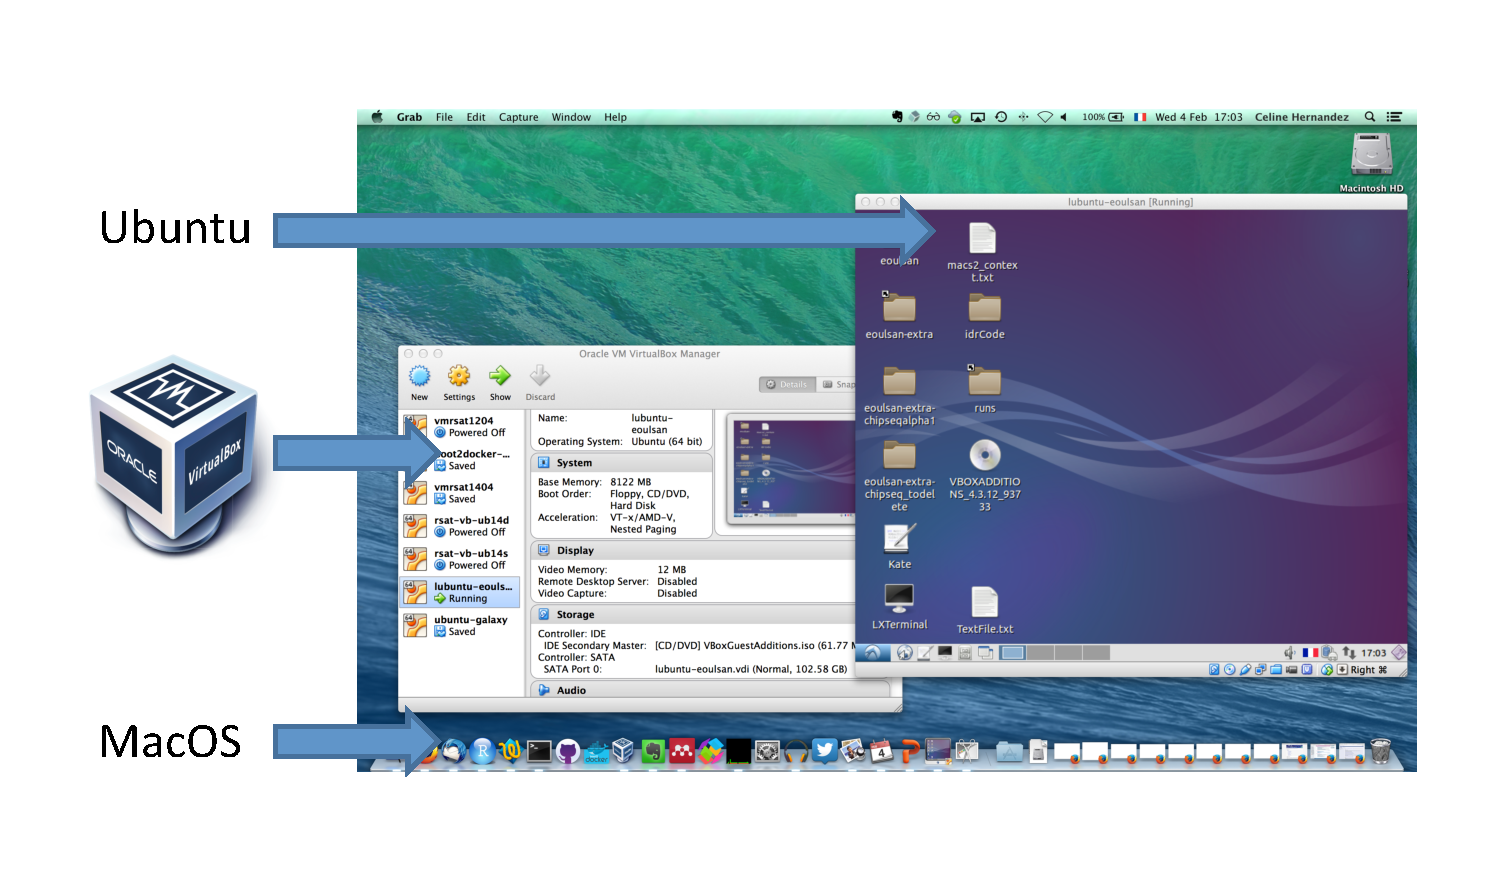
\includegraphics[width=12cm]{02_encapsulation/figures/virtual_machine_illus.pdf}

\end{frame}

%------------------------------------------------------------
\begin{frame}{Encapsulation : hardware virtualisation}
\begin{columns}

\column{0.5\textwidth}
\includegraphics[width=6cm]{02_encapsulation/figures/install_firefox.pdf}

\column{0.5\textwidth}
Idea: use virtual machines

Pros:  transferable independent environments

Cons:
\begin{itemize}
  \item Redundancy between VMs
  \item Heavy to set up
  \item No automation
\end{itemize}

\end{columns}
\end{frame}

%------------------------------------------------------------
\begin{frame}{Encapsulation : OS virtualisation}
\begin{columns}

\column{0.5\textwidth}
\includegraphics[width=6cm]{02_encapsulation/figures/install_firefox.pdf}

\column{0.5\textwidth}
Idea: "trick" applications into believing that they are in a different OS than the host's

Avoid redundancy.

\end{columns}
\end{frame}

%------------------------------------------------------------
\begin{frame}{Encapsulation : OS virtualisation}

\centering\includegraphics[width=12cm]{02_encapsulation/images/encapsulation_reproducibility_scale.png}

Practical Computational Reproducibility in the Life Sciences - Björn Grüning et al (2018) 

\end{frame}


%------------------------------------------------------------
\subsection{What is Docker?}

%------------------------------------------------------------
\begin{frame}{What is Docker?}

Docker is not very “old”
\begin{itemize}
  \item First commit January 2013
  \item First version March 2013
  \item Version 1.0 in June 2014
\end{itemize}

But its adoption was fast
\begin{itemize}
  \item Officially packaged in Ubuntu since 2014 (v14.04) 
\end{itemize}

\end{frame}

%------------------------------------------------------------
\begin{frame}{What is Docker?}

\begin{columns}

\column{0.5\textwidth}

\centering Image

\centering\includegraphics[width=4cm]{02_encapsulation/images/docker_images_illus.png}

\begin{itemize}
  \item Set of libraries and functions
  \item Fixed. Cannot be modified
  \item Can be stored/shared online
  \item Can be automatically built
\end{itemize}

\column{0.5\textwidth}

\centering Container

\centering\includegraphics[width=4cm]{02_encapsulation/images/docker_containers_illus.png} 

\begin{itemize}
  \item "Active image"
  \item Can be modified (interactive)
  \item Can be turned into an image
  \item One image, many containers
\end{itemize}

\end{columns}

\end{frame}

%------------------------------------------------------------
\begin{frame}{What is Docker?}

\centering\includegraphics[width=12cm]{02_encapsulation/images/docker_architecture.pdf}

(https://docs.docker.com/get-started/overview/)
\end{frame}

%------------------------------------------------------------
\begin{frame}{What is Docker?}

DockerHub

\centering\includegraphics[width=12cm]{02_encapsulation/images/docker_dockerhub_offrep.png}

(https://hub.docker.com/)
\end{frame}

%------------------------------------------------------------
\begin{frame}{What is Docker?}

Usermade images (1/2)

\centering\includegraphics[width=12cm]{02_encapsulation/images/docker_dockerhub_gpc.png}

(https://hub.docker.com/u/genomicpariscentre/)
\end{frame}

%------------------------------------------------------------
\begin{frame}{What is Docker?}

Usermade images (2/2)

Be critical!

\centering\includegraphics[width=10cm]{02_encapsulation/images/docker_dockerhub_gpc_samtools.png}

(https://hub.docker.com/r/genomicpariscentre/samtools/)
\end{frame}

%------------------------------------------------------------
\begin{frame}{What is Docker?}

\centering\includegraphics[width=12cm]{02_encapsulation/images/docker_architecture.pdf}

(https://docs.docker.com/get-started/overview/)
\end{frame}

%------------------------------------------------------------
\begin{frame}{What is Docker?}

Other commands :

\begin{itemize}
  \item docker images : list images available locally
  \item docker ps : status of containers
  \item docker rm : delete a container
  \item docker rmi : delete an image
  \item ...
\end{itemize}

(More details during the practical session.)

\end{frame}

%------------------------------------------------------------
\begin{frame}{Encapsulation : OS virtualisation}
\begin{columns}

\column{0.5\textwidth}
\includegraphics[width=6cm]{02_encapsulation/figures/install_firefox.pdf}

\column{0.5\textwidth}
OS virtualisation vs hardware virtualisation

Pros:
\begin{itemize}
  \item Speed 
  \begin{itemize}
    \item Installation is faster
    \item No boot time
  \end{itemize}
  \item Lightweight
  \begin{itemize}
    \item Minimal base OS
    \item Minimal libraries and application set
  \end{itemize}
  \item Easy sharing of applications
\end{itemize}

\end{columns}
\end{frame}

%------------------------------------------------------------
\begin{frame}{Encapsulation : OS virtualisation}
\begin{columns}

\column{0.5\textwidth}
\includegraphics[width=6cm]{02_encapsulation/figures/install_firefox.pdf}

\column{0.5\textwidth}

Cons:
\begin{itemize}
  \item Needs root access (Singularity)
  \item Changes of policies of the Docker company
\end{itemize}

\end{columns}
\end{frame}


%------------------------------------------------------------
\begin{frame}{Docker policy}

\centering Update of the Docker Image retention policy (13/08/2020)

\includegraphics[width=7cm]{02_encapsulation/images/docker_image_retention_policy.png}

https://www.docker.com/pricing/retentionfaq

\end{frame}

%------------------------------------------------------------
\subsection{Practical session}

%-------------------------------------------
\begin{frame}{Practical session}

Practical session : Docker and Samtools.

See companion document.

\end{frame}

%-------------------------------------------
\begin{frame}{Practical session}
%-------------------------------------------
\begin{block}{Analysis workflow}
    \includegraphics[width=12cm]{01_introduction/images/FAIR_RNAseq_WF.png}\\
green=input, blue=tool
\end{block}
\footnotesize{
\begin{description}
    \item[fastqc] control quality of the input reads
    \item[bowtie2] reads mapping on the genome sequence
    \item[samtools] mapped reads selection $\&$ formatting
    \item[HTseq] count table of mapped reads on genes (annotations)
    \item[DEseq2] statistical analysis: genes list having differential expression
\end{description}
}
\end{frame}

%------------------------------------------------------------
\begin{frame}{Practical session}
Savoir FAIRe

\begin{itemize}
  \item (Installation de Docker)
  \item Learn the structure of a Docker command
  \item Pull a pre-defined image available on the DockerHub
  \item Start a container
  \item Bonus: build a Dockerfile
\end{itemize}
\end{frame}

%------------------------------------------------------------
% Une ressource sympa : https://xataz.developpez.com/tutoriels/utilisation-docker/